\chapter{Self Supervised Learning} \label{chap:self-supervised-learning}

In recent years, the field of artificial intelligence has progressed leaps and bounds at an astronomical rate. 
However, the vast majority of progress has been made in the \textbf{supervised} domain, where we have massive amounts of carefully labelled data available. Such models perform extremely well in the singular task for which they were trained.

However, the reality is such that we cannot always possess massive amounts of labelled data for a given task at hand.
There are some tasks for which there are simply not enough high-quality labelled data. Examples of such tasks include modelling esoteric languages for which we do not have enough resources or several image classification tasks in the medical domain.
Furthermore, supervised learning has shown us that it is constrained when it comes to building easily generalisable models.
The idea is that if AI systems can gain a more nuanced understanding of the reality beyond what is specified and constrained by training labels, they will ultimately be closer to human-level understanding.
\begin{figure}[th]
    \centering
    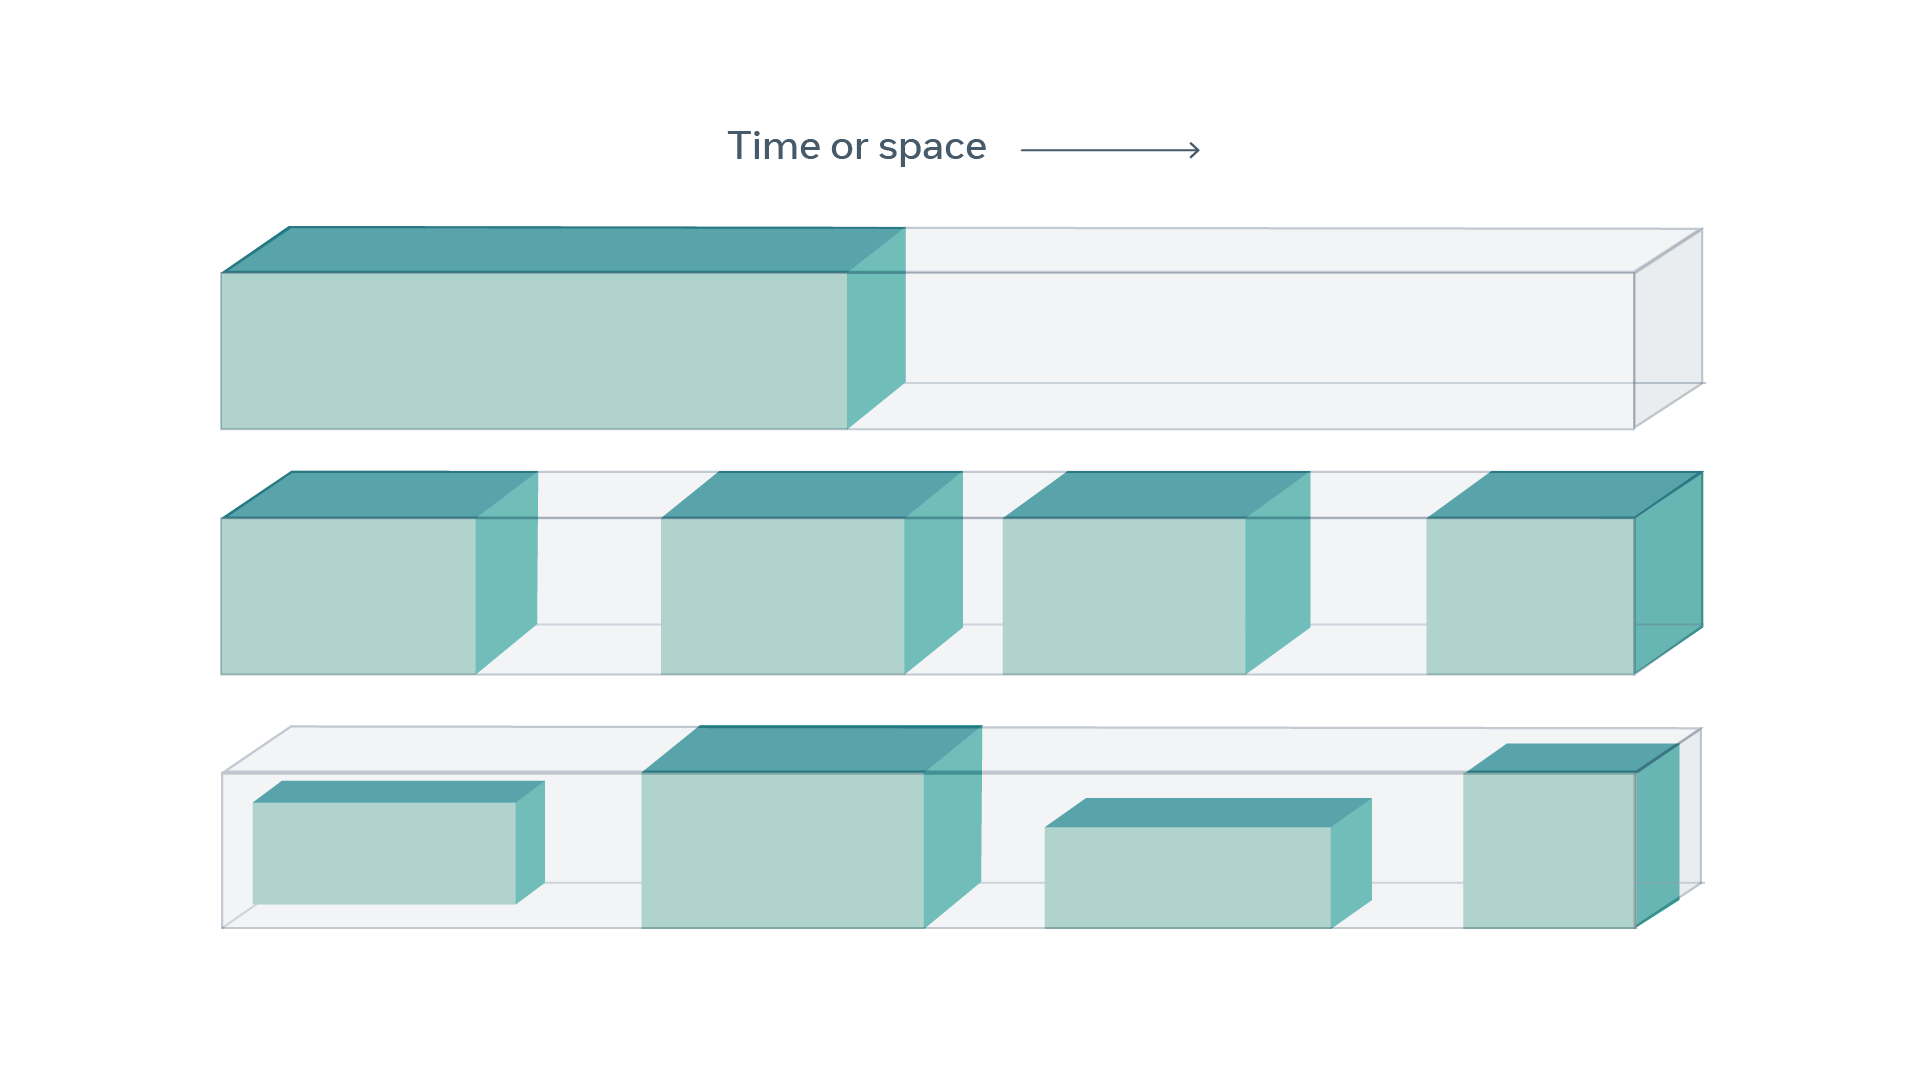
\includegraphics[width=\linewidth]{chapters/assets/ssl_figs/ssl.png}
    \caption{In self-supervised learning, the system is trained to predict hidden parts of the input (in \textcolor{gray}{gray}) from visible parts of the input (in \textcolor{tudelft-turquoise}{green}).}
    \label{fig:ssl-idea}
\end{figure}

Self-supervised learning (SSL) is currently the most promising form of \textbf{unsupervised learning} alternative to supervised learning, which is perhaps capable of guiding AI systems to learn general knowledge and an approximate form of common sense. Self-supervision typically involves formulating a specialised supervised task to predict only a subset of information from the rest (see \Cref{fig:ssl-idea}). This idea has been used extensively in language modelling. The default task of a language model is to predict the next word given a sequence of words (or a partial sentence). We then use the trained model to help us solve another related task. This concept is called \textbf{transfer learning}, where we the \textbf{pre-train} the model on a large dataset, then save the weights and apply it to another possibly related problem. Often we may also want to \textbf{fine-tune} the saved model weights by training it for a few epochs at a slow learning rate on the dataset pertinent to the new problem.
The pre-training can be either supervised or unsupervised; however, we shall only be focusing on the unsupervised (self-supervised) aspect. It is also worth noting that most self-supervised training schemes focus on \textbf{representation learning}, and we shall cover this in a bit more detail in \Cref{sec:repr-learning}.

SEER \parencite{Goyal2021}, a research project from Meta AI, made use of SWaV \parencite{caron2020unsupervised} to train a computer vision model that has outperformed state-of-the-art supervised models on tasks such as image classification, object detection and image segmentation. SEER's performance demonstrates quite conclusively that SSL methods can excel at computer vision tasks while learning generalisable features. The work done on SEER parallels the work being done in the NLP field for a while now, where state-of-the-art models frequently use billions of parameters and train using SSL methods on huge datasets.


\section{Representation Learning} \label{sec:repr-learning}
The performance of machine learning methods is highly dependent on the choice of data representation (or features) on which they are applied. For that reason, much of the actual effort in deploying machine learning algorithms goes into the design of preprocessing pipelines and data transformations that result in a representation of the data that can support effective machine learning. Our goal with representation learning is to allow the model to learn robust representations with minimal human interference.

Representation learning aims to train machine learning algorithms to learn useful representations, e.g. interpretable representations, useful latent features, or allow transfer learning to be used. 
Deep neural networks can be considered representation learning models that typically encode information that is projected into a different subspace. These representations are then usually passed on to a linear classifier to, for instance, train a classifier. 
\begin{figure}[h]
    \centering
    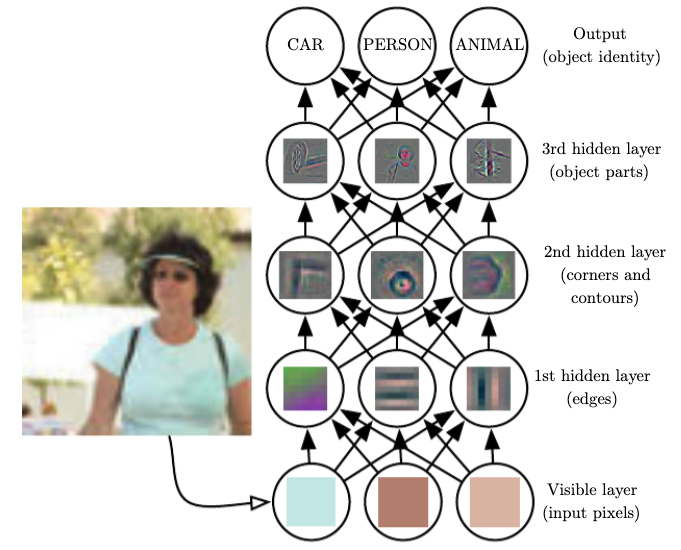
\includegraphics[scale=0.4]{chapters/assets/ssl_figs/ssl_rep_learning_images.png}
    \caption{Deep neural networks combine simple concepts to learn representations and derive complex structures in a hierarchical pipeline. Each layer refines  information from the previous layer. Finally, the  classifier takes the transformed representation and draws boundaries between classes. See \Cref{fig:feature-viz} for more.}
    \label{fig:small-cnn-features}
\end{figure}

At a high level, a network has two components:
\begin{enumerate}
    \item an encoder (also called a feature extractor in \Cref{fig:cnn-overview})
    \item and a linear classifier.
\end{enumerate}
The encoder transforms the input data and projects them into a subspace that we refer to as \textbf{latent space}. Then the representation (output of the encoder) is passed to a linear classifier. Typically, in a supervised setting, we would like to map representations to labels, which a classical classifier would do. 
However, representation learning aims at mapping representations to other representations. These learned representations are often dense and compact; they can also generalise to similar data modalities. In other words, these representations can \textbf{transfer} well for other tasks and have been the principal method for solving problems in which data annotations are hard or even impossible to obtain. The learned representations are stored in the weights of the model, \Cref{fig:small-cnn-features} shows a small example where the hidden layers have learnt to recognise specific components of an image. One can save these learnt weights and reuse them for other tasks. 

\section{Self-supervision with Images} \label{sec:self-sup-with-images}

\begin{figure}
    \centering
    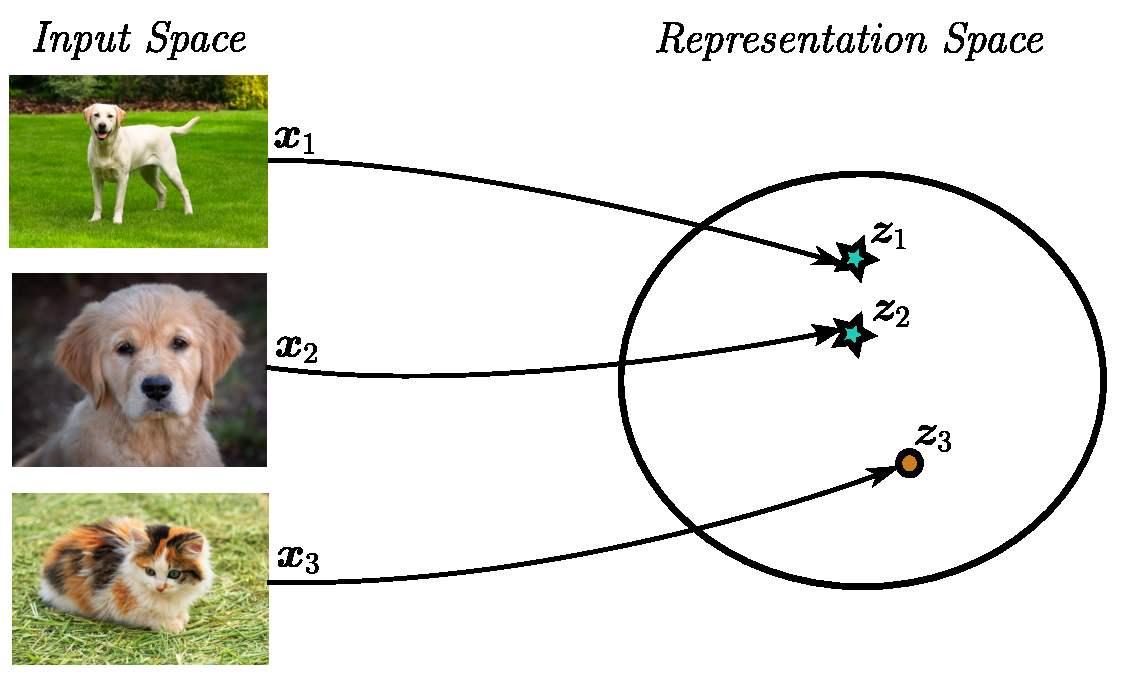
\includegraphics[scale=0.4]{chapters/assets/ssl_figs/representation_space.pdf}
    \caption{We have three images $\symbfit{x}_1, \symbfit{x}_2$ and $\symbfit{x}_3$. The first two images depict a dog, and the third image depicts a cat. The network should ideally learn to place the dogs closer together ($\symbfit{z}_1$ and $\symbfit{z}_2$) in the representation space and the cat ($\symbfit{z}_3$) farther away from the dogs.}
    \label{fig:my_label}
\end{figure}

As mentioned above in this text, self-supervision usually involves formulating a specialised supervised task; this task is also called a \textbf{pretext task}. However, we normally do not care about the performance of the model on this artificial task. Rather, we are more concerned with the intermediate learned representations with the hope that this representation carries with it good semantic or structural meanings that be beneficial to a wide variety of real word tasks.

For example, we might rotate images at four random angles and train a model to predict how each image has been rotated. Here, the task of predicting rotations is the pretext task, so the actual accuracy on this task is irrelevant to us \parencite{gidaris2018unsupervised}. Instead, we expect the model to learn high-quality latent representations that are useful for other real-world tasks.

However, this is not the only way, and in the next section we shall discuss one of the most popular techniques in this space.

\section{Contrastive Representation Learning}\label{sec:contrastive-learning}
The goal of contrastive representation learning is to learn a feature subspace in which similar (positive) pairs of data items stay close to each other while dissimilar (negative) pairs are farther apart. Contrastive learning can be applied to both supervised and unsupervised settings. For unsupervised learning, contrastive learning remains one of the most powerful approaches to self-supervised learning.

When working in a supervised setting, it is easy to find positive pairs of the data; one only needs to fetch images that are associated with the same true label. However, in an unsupervised setting, we have no such label information; therefore, we must get creative in order to teach the network what constitutes as a positive pair of images. This brings us to one of the most intuitive techniques, SimCLR \parencite{chen2020simple}.

\subsection{SimCLR} \label{ssec:simclr}

\begin{figure}[th]
\centering
\begin{subfigure}{.19\textwidth}
  \centering
  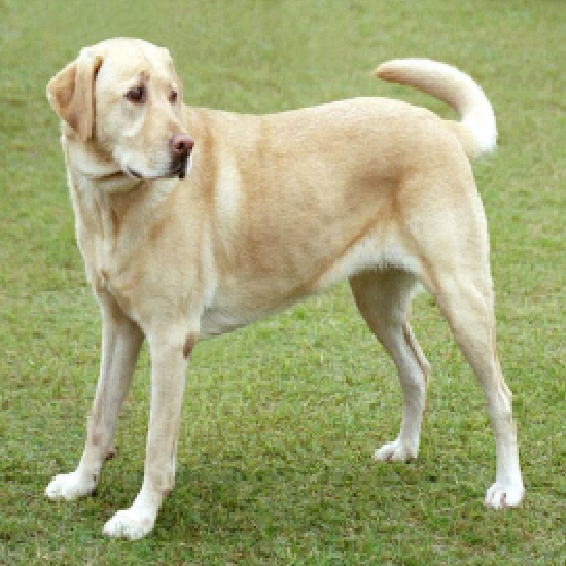
\includegraphics[width=0.9\linewidth]{chapters/assets/ssl_figs/transforms/img_original.pdf}
  \caption{Original}
\end{subfigure}\begin{subfigure}{.19\textwidth}
  \centering
  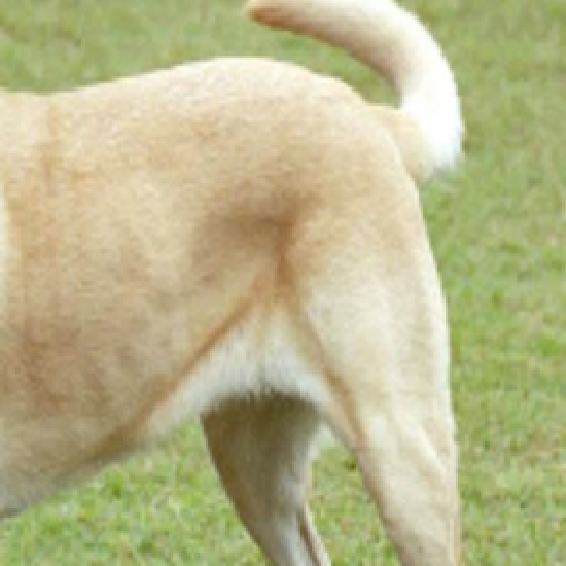
\includegraphics[width=0.9\linewidth]{chapters/assets/ssl_figs/transforms/img_crop1.pdf}
  \caption{Crop and resize}
\end{subfigure}\begin{subfigure}{.19\textwidth}
  \centering
  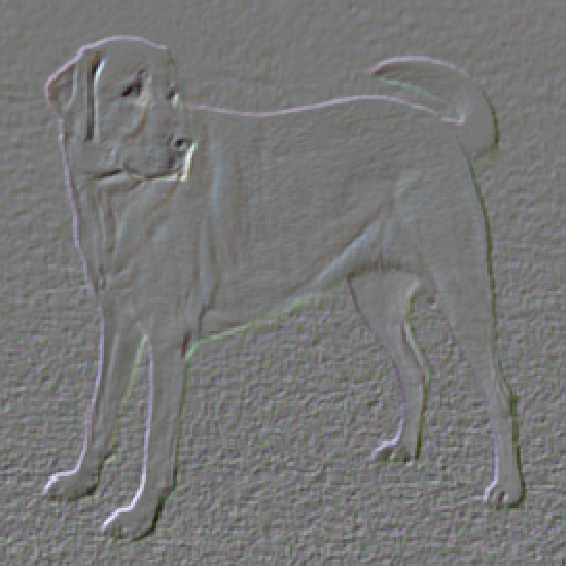
\includegraphics[width=0.9\linewidth]{chapters/assets/ssl_figs/transforms/img_sobel.pdf}
  \caption{Sobel filtering}
\end{subfigure}\begin{subfigure}{.19\textwidth}
  \centering
  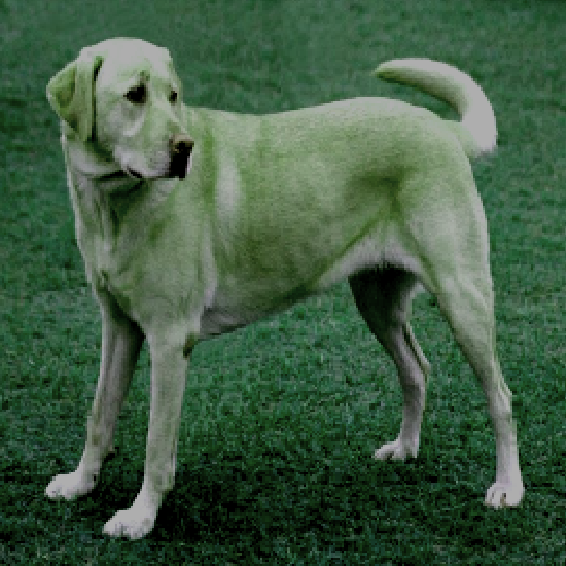
\includegraphics[width=0.9\linewidth]{chapters/assets/ssl_figs/transforms/img_color1.pdf}
  \caption{Color distort. (drop)}
\end{subfigure}\begin{subfigure}{.19\textwidth}
  \centering
  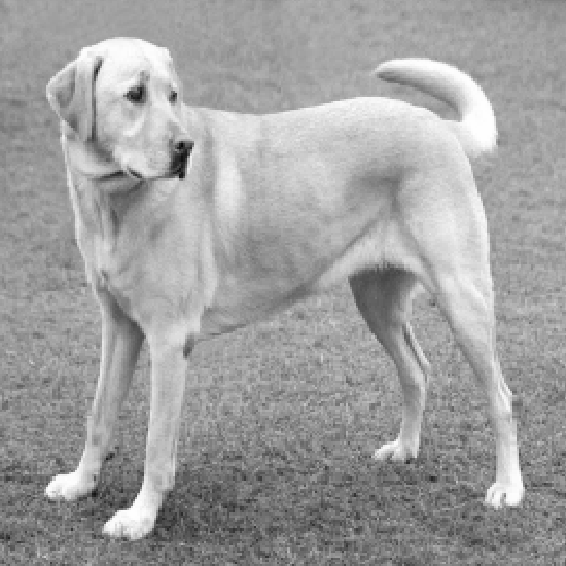
\includegraphics[width=0.9\linewidth]{chapters/assets/ssl_figs/transforms/img_color.pdf}
  \caption{Color distort. (jitter)}
\end{subfigure}\\
\begin{subfigure}{.19\textwidth}
  \centering
  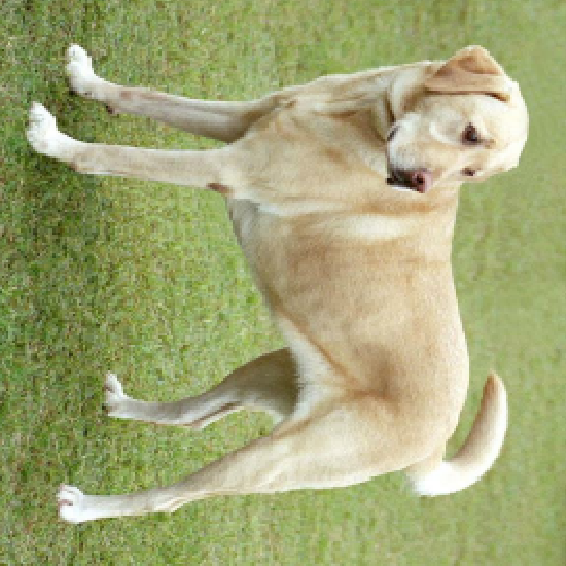
\includegraphics[width=0.9\linewidth]{chapters/assets/ssl_figs/transforms/img_rotate.pdf}
  \caption{Rotate {\tiny$\{90\degree,180\degree,270\degree\}$}}
\end{subfigure}\begin{subfigure}{.19\textwidth}
  \centering
  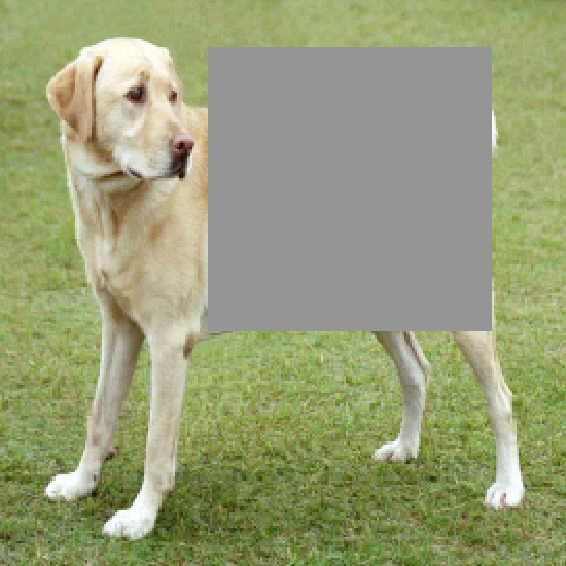
\includegraphics[width=0.9\linewidth]{chapters/assets/ssl_figs/transforms/img_cutout.pdf}
  \caption{Cutout}
\end{subfigure}\begin{subfigure}{.19\textwidth}
  \centering
  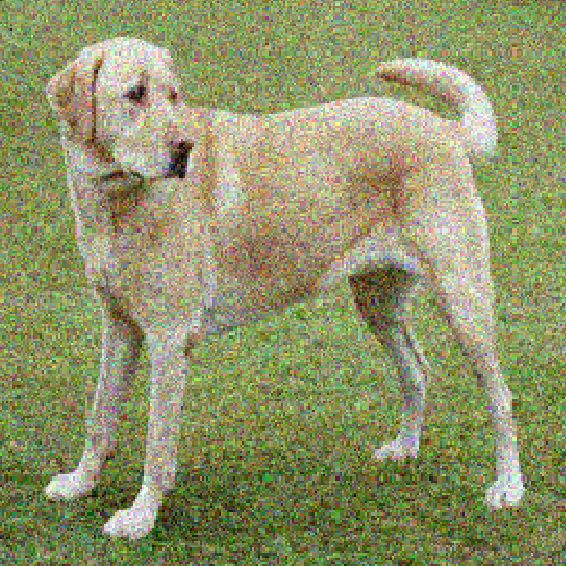
\includegraphics[width=0.9\linewidth]{chapters/assets/ssl_figs/transforms/img_noise.pdf}
  \caption{Gaussian noise}
\end{subfigure}\begin{subfigure}{.19\textwidth}
  \centering
  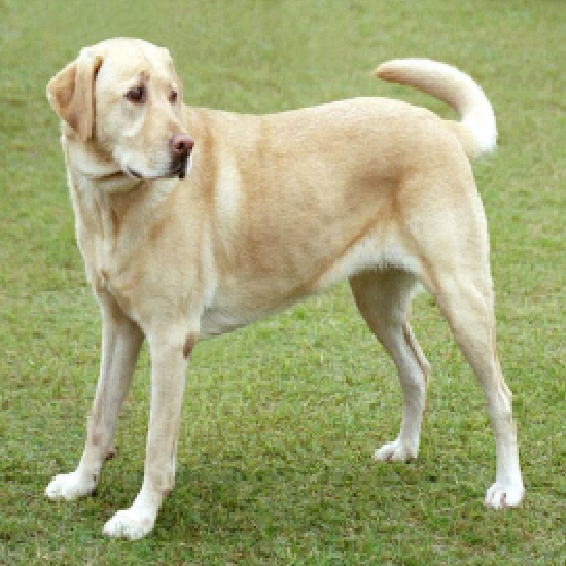
\includegraphics[width=0.9\linewidth]{chapters/assets/ssl_figs/transforms/img_gblur.pdf}
  \caption{Gaussian blur}
\end{subfigure}\begin{subfigure}{.19\textwidth}
  \centering
  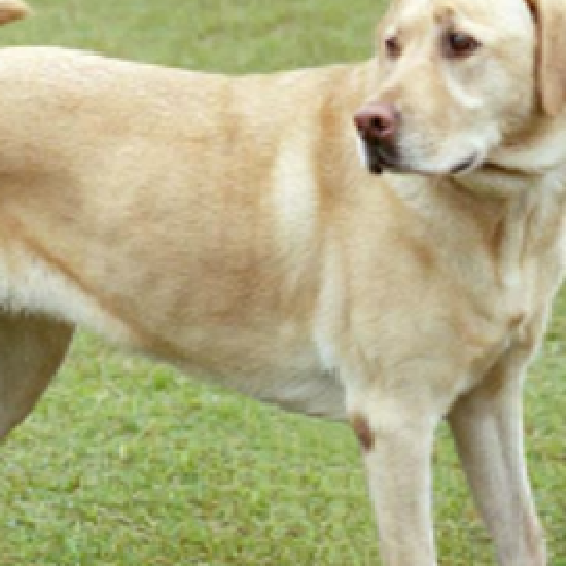
\includegraphics[width=0.9\linewidth]{chapters/assets/ssl_figs/transforms/img_crop.pdf}
  \caption{Crop, resize (and flip)}
\end{subfigure}\vskip -0.05in
\caption{Illustrations of data augmentation operators. (Original image cc-by: Von.grzanka)}
\label{fig:simclr-data_aug}
\end{figure}

The idea behind SimCLR is quite simple and elegant. An image $\symbfit{x}$ is randomly sampled from the dataset, and then two random transformations are applied to the image to obtain two augmented images $\symbfit{x}_i$ and $\symbfit{x}_j$. Each image is passed through the encoder to obtain the representations $\symbfit{z}_i$ and $\symbfit{z}_j$, respectively. The goal here is to maximise the similarity between $\symbfit{z}_i$ and $\symbfit{z}_j$, see \Cref{fig:simclr} for a small overview of SimCLR. \Cref{fig:simclr-data_aug} shows a few examples of the type of image transformations used by SimCLR.

In order to train the network to bring the said representations closer, we first measure the similarity between them using a \textbf{similarity metric} such as cosine similarity or Euclidean distance. The cosine similarity metric between $\symbfit{z}_i$ and $\symbfit{z}_j$ is given as
\begin{equation}
\label{eqn:simclr-cosine-sim}
s_{i, j}=\frac{\symbfit{z}_{i}^{\top} \symbfit{z}_{j}} {\left(\left\|\symbfit{z}_{i}\right\|\left\|\symbfit{z}_{j}\right\|\right)}
\end{equation}

\highlight[comment=maybe add an example of the mini batch]{We} calculate the pairwise cosine similarity between each augmented image in a mini-batch using \Cref{eqn:simclr-cosine-sim}. In the ideal case, the similarity between all \textit{postive} pairs must be high and low between all \textit{negative} pairs.

Next, we use pairwise cosine similarities to calculate the loss. The loss is called \textbf{NT-Xent} (normalised temperature-scaled cross-entropy loss) or NCE (noise contrastive estimator) and is given as
\begin{equation}
\ell(i, j)=-\log \frac{\exp \left(s_{i, j} / \tau\right)}{\sum_{k=1}^{2 n} \mathbb{1}_{[k \neq i]} \exp \left(s_{i, k} / \tau\right)}
\label{eqn:nt-xent}
\end{equation}
where $\tau$ is the temperature scaling factor. The reader is urged to recognise the similarities between \Cref{eqn:nt-xent} and \Cref{eqn:std-softmax}. \Cref{eqn:nt-xent} is indeed just the normal $\operatorname{softmax}$ (\Cref{eqn:std-softmax}) with an additional temperature scaling factor.

Normally a mini-batch of $n$ samples is randomly sampled, since the contrastive pretext task is defined on pairs of augmented images derived from the minibatch, it results in a total of $2n$ data points. The negative samples are not sampled explicitly. Instead, given a positive pair, the other $2(n-1)$ augmented samples in a mini-batch are treated as negative samples.

You can choose $\tau$ to be any value; higher values of $\tau$ will lead to a \textquote{softer} output distribution of probabilities, for example, $\left[0.01,0.01,0.98\right]$.
As $\tau$ approaches $0$, it will lead to a distribution \textquote{sharper}, for example, $\left[0.2,0.2,0.6\right]$.
A distribution of \textquote{softer} implies that the model is less confident in its predictions, while \textquote{sharper} implies that the model is very confident.

A low temperature ($<1$) discourages predictions from collapsing to a uniform distribution, which is undesirable. When we talk about collapse, we are talking about \textbf{representation collapse}. Representation collapse is a phenomenon where in the network outputs the same representation regardless of the input, as one can imagine if every pair of images has the same representation, the loss would be incredibly low. However, if the network returns the same representation for all input, its not very useful for downstream tasks that require the features to be discriminative and have semantic information.

\begin{tcolorbox}[title=Intuition for Temperature]
The temperature parameter penalises the larger logits more than the smaller logits. The exponential function is an \textquote{increasing function}. So, if a term is already large, penalising it by a small amount would make it much smaller (\% wise) than if that term were small.
\end{tcolorbox}

\begin{figure}
    \centering
    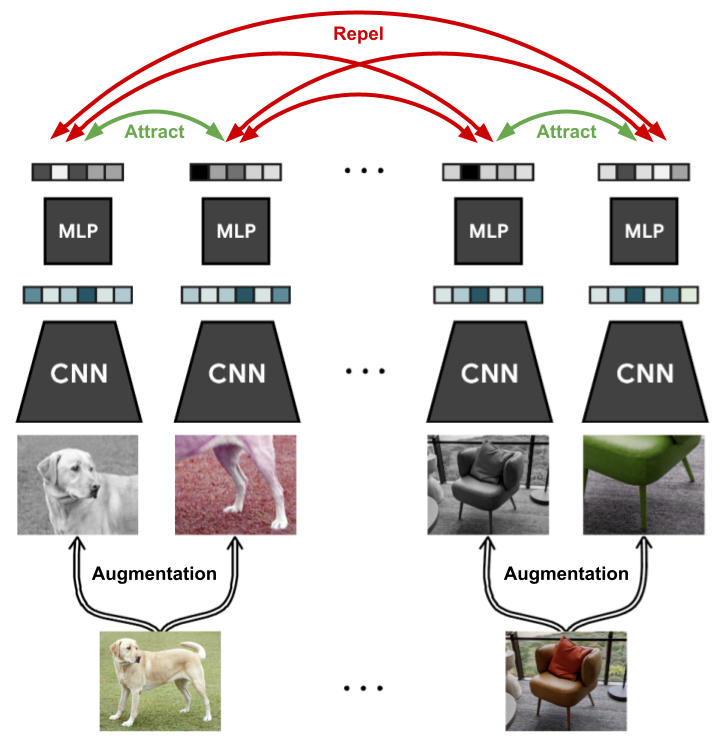
\includegraphics[scale=0.4]{chapters/assets/ssl_figs/simclr_contrastive_learning.png}
    \caption{SimCLR works by augmenting an image twice and ensuring their representations are close to each other while being farther away from representations of other augmented images.}
    \label{fig:simclr}
\end{figure}